\section{Output}

PyLith currently supports output to HDF5/Xdmf and VTK files, which can
be imported directly into a number of visualization tools, such as
ParaView, Visit, and MayaVi. The HDF5 files can also be directly
accessed via Matlab and Python modules, such as h5py and
PyTables. PyLith v3.x supports output of the solution subfields (see
Section \vref{sec:solution:observers}) all auxiliary fields
(material properties, boundary condition parameters, and fault interface
parameters, etc.) and fields derived from the auxiliary field and/or
solution, such as stress and stress.

HDF5 writer provides parallel binary output, whereas the VTK writer
provides serial ASCII output. Additionally, with the VTK writer each
time step is written to a separate file; the HDF5 writer puts all
information for a given domain, boundary condition, or fault interface
into a single file.


\subsection{Physics Observer (\object{OutputPhysics})}

Analogous to the \object{OutputSoln} objects discussed in Section
\vref{sec:solution:observers} for output of the solution, the physics
objects (material, boundary conditions, and fault interfaces) have
\object{OutputPhysics} objects to provide output of the solution,
properties, state variables, etc. 

The parameters for the \object{OutputPhysics} are:
\begin{inventory}
  \propertyitem{info\_fields}{List of auxiliary subfields to observer/output (default=all which will output all of the subfields);}
  \propertyitem{data\_fields}{List of solution subfields to observer/output (default=all which will output all of the subfields);}
  \facilityitem{writer}{Writer for data (default=\object{DataWriterHDF5});}
  \facilityitem{trigger}{Trigger defining how often output is written (default=\object{OutputTriggerStep}); and}
  \facilityitem{field\_filter}{Filter for output fields (default=\object{FieldFilterNone}).}
\end{inventory}

\begin{cfg}[\object{PhysicsOutput} parameters in a \filename{cfg} file]
<h>[pylithapp.problem.materials.elastic.observers.observer]</h>
<p>writer.filename</p> = output/step01-elastic.h5
<f>field_filter</f> = pylith.meshio.FieldFilterNone
\end{cfg}

\subsection{Output Field Filter (\facility{field\_filter})}

Sometimes fields may not be in the form a user wants. For example, the
displacement solution subfield may have a basis order of 2 with
degrees of freedom associated with edges, which is incompatible with
most visualization packages that require information be provided with
a basis order of 1 (vertex data) or 0 (cell data). The
\facility{field\_filter} facility of the \object{OutputPhysics} object
allows passing a field through a ``filter'' to yield the desired form
of the output. The default filter is \object{FieldFilterNone}, which
simply passes the input field on to the \facility{writer} for
output. The \object{FieldFilterProject} object provides the ability to
project the input field to a lower basis order.

\subsubsection{Projecting to lower basis order (\object{FieldFilterProject})}

This filter projects a field to a lower basis order. It is most often
used to reduce the basis order of solution subfields, e.g,,
displacement, to a basis order of 1 from a basis order of 2, so that
the solutino field can be visualized in common ParaView, etc.
The \object{fieldFilterProject} property is:
\begin{inventory}
  \propertyitem{basis\_order}{Basis order of the projected field (default=1).}
\end{inventory}

\begin{cfg}[Using \object{FieldFilterProject} with solution output in
  a \filename{cfg} file]
<h>[pylithapp.problem.solution_observers.domain]</h>
<p>writer.filename</p> = output/step01-domain.h5
<f>field_filter</f> = pylith.meshio.FieldFilterProject
<p>field_filter.basis_oder</p> = 0
\end{cfg}


\subsection{Data Writers (\facility{writer})}

\subsubsection{VTK Output (\object{DataWriterVTK})}

PyLith writes legacy (non-XML) VTK files. These are simple files with
vertex coordinates, the mesh topology, and fields over vertices and/or
cells. Each time step is written to a different file. The time stamp
is included in the filename with the decimal point removed. This allows
automatic generation of animations with many visualization packages
that use VTK files. The default time stamp is the time in seconds,
but this can be changed using the normalization constant to give a
time stamp in years, tens of years, or any other value.


The parameters for the VTK writer are:
\begin{inventory}
\propertyitem{filename}{Name of VTK file.}
\propertyitem{time\_format}{C-style format string for time stamp in filename.
The decimal point in the time stamp will be removed for compatibility
with VTK visualization packages that provide seamless animation of
data from multiple VTK files.}
\propertyitem{time\_constant}{Value used to normalize time stamp in VTK files
(default is 1.0 s).}
\end{inventory}

\userwarning{We strongly discourage use of using VTK output. It is slow,
  inefficient, and not easily read from post-processing scripts. We
  strongly recommwnd using HDF5 output instead, which is the default
  starting in PyLith v3.0.0.}

\subsubsection{HDF5/Xdmf Output (\object{DataWriterHDF5}, \object{DataWriterHDF5Ext})}
\label{sub:HDF5/Xdmf-Output}

HDF5 files provide a flexible framework for storing simulation data
with datasets in groups logically organized in a tree structure analogous
to files in directories. HDF5 output offers parallel, multi-dimensional
array output in binary files, so it is much faster and more convenient
than the VTK output which uses ASCII files and separate files for
each time step. Standards for organizing datasets and groups in HDF5
files do not exist for general finite-element software in geodynamics.
Consequently, PyLith uses its own simple layout show in Figure \vref{fig:hdf5:layout}.
In order for visualization tools, such as ParaView, to determine which
datasets to read and where to find them in the hierarchy of groups
within the HDF5 file, we create an Xdmf (eXtensible Data Model and
Format, \url{www.xdmf.org}) metadata file that provides this information.
This file is written when PyLith closes the HDF5 file at the end of
the simulation. In order to visualize the datasets in an HDF5 file,
one simply opens the corresponding Xdmf file (the extension is \filename{xmf})
in ParaView or Visit. The Xdmf file contains the relative path to
the HDF5 file so the files can be moved but must be located together
in the same directory. 

\important{The Xdmf format supports
representation of two- and three-dimensional coordinates of points,
scalar fields, and three-dimensional vector and tensor fields but
not two-dimensional vector or tensor fields. Consequently, for two-dimensional
vector fields we build a three-component vector from the two-component
vector (x and y components) and a separate zero scalar field (z component).
For tensor fields, we create a scalar field for each of the tensor
components, adding the component as a suffix to the name of the field.}

\begin{figure}[htbp]
  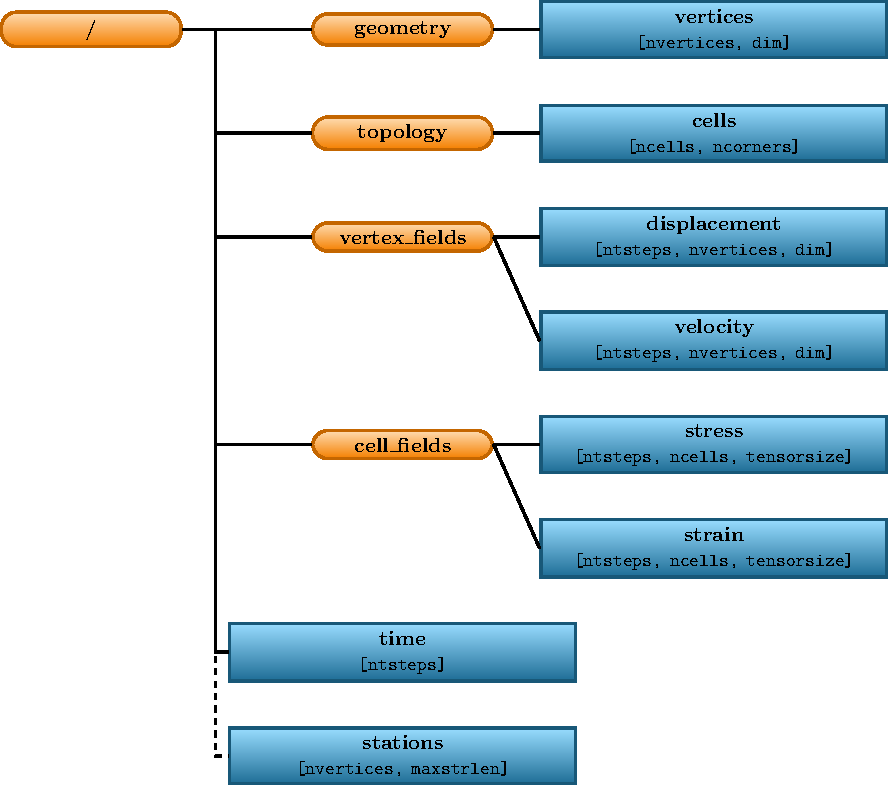
\includegraphics{runpylith/figs/hdf5layout}
  \caption{General layout of a PyLith HDF5 file. The orange rectangles
    with rounded corners identify the groups and the blue rectangles
    with sharp corners identify the datasets. The dimensions of the
    data sets are shown in parentheses. Most HDF5 files will contain
    either \texttt{vertex\_fields} or \texttt{cell\_fields} but not
    both.}
 \label{fig:hdf5:layout}
\end{figure}

See Table \vref{tab:materials:statevars} in Section
\vref{sec:material:parameters} for a table of component values for
tensor output in HDF5 files. To avoid confusion about the ordering of
components for tensor data, we separate the components in the Xdmf
file.

The \object{DataWriterHDF5} and \object{DataWriterHDF5Ext} property is:
\begin{inventory}
  \propertyitem{filename}{Name of HDF5 file (default=output.h5; the
    Xdmf filename is generated from the same prefix).}
\end{inventory}

\begin{cfg}[\object{DataWriterHDF5Ext} parameters in a \filename{cfg} file]
<h>[pylithapp.timedependent.domain.output]</h>
<p>output_freq</p> = time_step
<p>time_step</p> = 1.0*yr
<p>cell_data_fields</p> = [displacement, velocity]
<f>writer</f> = pylith.meshio.DataWriterHDF5Ext
<p>writer.filename</p> = dislocation.h5
\end{cfg}
In this example, we change the writer from the default VTK writer to
the HDF5 writer with external datasets (\object{DataWriterHDF5Ext})
for output over the domain.

HDF5 files do not contain self-correcting features that allow a file
to be read if part of a dataset is corrupted. This type of error can
occur if a job terminates abnormally in the middle or at the end of a
simulation on a large cluster or other parallel machine. Fortunately,
HDF5 also offers the ability to store datasets in external binary
files with the locations specified by links in the HDF5 file. Note
that the use of external data files results in one data file per
dataset in addition to the HDF5 and Xdmf files. The external data
files use the name of the HDF5 file with the dataset name added to the
prefix and the \filename{h5} suffix replaced by \filename{dat}. The
HDF5 files include relative paths to the external data files, so these
files can also be moved, but they, too, must be kept together in the
same directory. This provides a more robust method of output because
one can generate an HDF5 file associated with the uncorrupted portions
of the external data files should an error occur. Currently, PyLith
does not include a utility to do this, but we plan to add one in a
future release. Thus, there are two options when writing PyLith output
to HDF5 files: (1) including the datasets directly in the HDF5 files
themselves using the \object{DataWriterHDF5} object or (2) storing the
datasets in external binary files with just metadata in the HDF5 files
using the \object{DataWriterHDF5Ext} object. Both methods provide
similar performance because they will use MPI I/O if it is available.

\userwarning{Storing the datasets within the HDF5 file in a parallel
  simulation requires that the HDF5 library be configured with the
  \commandline{-{}-enable-parallel} option. The binary PyLith packages
  include this feature and it is a default setting in building HDF5
  via the PyLith Installer.}

Accessing the datasets for additional analysis or visualization is
nearly identical in the two methods because the use of external data
files is completely transparent to the user except for the presence
of the additional files. Note that in order for ParaView to find the
HDF5 and external data files, it must be run from the same relative
location where the simulation was run. For example, if the simulation
was run from a directory called ``work'' and the HDF5/Xdmf files
were written to ``work/output'', then ParaView should be run from
the ``work'' directory. See Table \vref{tab:materials:statevars}
in Section \vref{sec:material:parameters} for a table of component
values for tensor output.

\begin{cfg}[Selecting \object{DataWriterHDF5Ext} in a \filename{cfg}
  file]
<h>[pylithapp.problem]</h>
<f>solution_observers</f> = [domain]
<f>solution_observers.domain>/f> = pylith.mehsio.DataWriterHDF5Ext

<h>[pylithapp.problem.solution_observers.domain]</h>
<p>writer.filename</p> = output/step01-domain.h5
\end{cfg}

\subsubsection{HDF5 Utilities}

HDF5 includes several utilities for examining the contents of HDF5
files. \filename{h5dump} is very handy for dumping the hierarchy,
dimensions of datasets, attributes, and even the dataset values to
stdout. 
\begin{shell}
# Dump the entire HDF5 file (not useful for large files).
$ h5dump mydata.h5

# Dump the hierarchy of an HDF5 file.
$ h5dump -n mydata.h5

# Dump the hierarchy with dataset dimensions and attributes.
$ h5dump -H mydata.h5

# Dump dataset 'vertices' in group '/geometry' to stdout.
$ h5dump -d /geometry/vertices mydata.h5
\end{shell}
We have also include a utility \filename{pylith\_genxdmf} (see Section
\vref{sec:pylith:genxdmf}) that generates an appropriate Xdmf file
from a PyLith HDF5 file. This is very useful if you add fields to
HDF5 files in post-processing and wish to view the results in ParaView
or Visit.


\subsection{Output Triggers (\facility{trigger})}
\newfeature{3.0}

By default PyLith will write the requested output after every time
step. In many cases we prefer to save the solution, state variables,
etc at a coarser temporal resolution. The \object{OutputTriggerStep}
controls the decimation of the output by time step, and the
\object{OutputTriggerTime} controls the decimation of the output via
time. For uniform time stepping these are equivalent.

\subsubsection{Decimate by time step (\object{OutputTriggerStep})}

\object{OutputTriggerStep} decimates the output by skipping a
user-specified number of time steps. The property is
\begin{inventory}
  \propertyitem{num\_skip}{Number of solution steps to skip between
    writes (default=0).}
\end{inventory}

  
\subsubsection{Decimate by time (\object{OutputTriggerTime})}

\object{OutputTriggerTime} decimates the output by skipping a
user-specified elasped time. The property is
\begin{inventory}
  \propertyitem{elapsed\_time}{Elasped time between writes (default=0.0*s).}
\end{inventory}
 
\usertip{Due to roundoff error in determining the simulation time over
  many time steps, a simulation may occasionally skip writing output
  unexpectedly when using \object{OutputTriggerTime}. The best
  workaround is to use an \property{elapsed\_time} that is a fraction
  of the time step size smaller than the desired elapsed time, such as
  0.9999*year instead of 1.0*year.}
  
% End of file
